\documentclass[11pt,twocolumn,letterpaper]{article}

\usepackage{cvpr}
\usepackage{times}
\usepackage{epsfig}
\usepackage{graphicx}
\usepackage{amsmath}
\usepackage{amssymb}
\usepackage[nottoc]{tocbibind}
\usepackage{hyperref}
\hypersetup{
    colorlinks=true,
    linkcolor=blue,
    filecolor=magenta,      
    urlcolor=cyan,
}

\cvprfinalcopy
\def\cvprPaperID{****} 
\def\httilde{\mbox{\tt\raisebox{-.5ex}{\symbol{126}}}}

\setcounter{page}{1}
\begin{document}

\title{Pose Space Deformation}

\author{Veronica Lee\\
\and
Yifan Wang\\
}

\maketitle

\begin{abstract}
Skeletal animation is a technique used for character animation in computer graphics, where a character is represented as a hierarchical model consisting of bones and skins enveloping the bones. Skinning methods focus on how to appropriately envelope the bones with a skin mesh. In this paper, we discuss the implementation and comparison of two example-based skinning methods: skeletal subspace deformation (SSD) and pose space deformation (PSD). We also discuss our attempt to compute joint weights using the pose samples.
\end{abstract}

\section{Introduction}

Skeletal animation is a technique used for character animation in computer graphics, where a character is represented as a hierarchical model consisting of bones and skins enveloping the bones. Skinning methods focus on how to appropriately envelope the bones with a skin mesh. There are three common approaches to skinning: 1) algorithmic, 2) physically-based, and 3) example-based. Purely algorithmic or physically-based skinning methods can have shortcomings because it is difficult to accurately model the complex biomechanics of skin deformation. Example-based methods require first creating a set of examples, but the results are likely to be more realistic.

Skeletal subspace deformation (SSD) \cite{magnenat1988joint} is a commonly used example-based method for skinning that uses a weighted transformation from the bind pose. Pose space deformation (PSD) \cite{lewis2000pose} is another example-based skinning method that  performs better than SSD, especially for poses at sharp angles. In this paper, we will discuss the implementation and comparison of SSD and PSD, primarily by following the implementation as described in \cite{rhee2006real}. We will also discuss our attempt to compute joint weights using the pose samples defined for PSD \cite{wang2002multi, mohr2003direct}.

\begin{figure}[t]
\begin{center}
\fbox{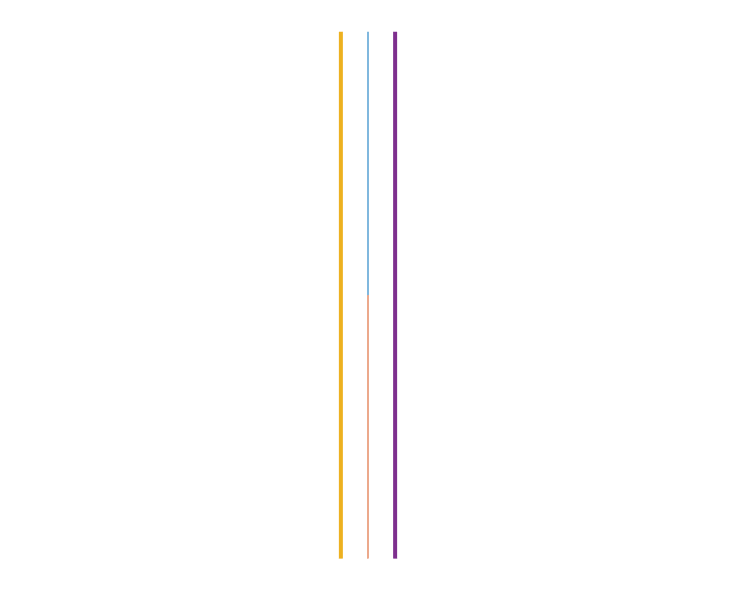
\includegraphics[width=0.6\linewidth]{bindpose.png}}
\end{center}
   \caption{The bind pose for SSD.}
\label{fig:long}
\label{fig:onecol}
\label{bind}
\end{figure}

%------------------------------------------------------------------------
\section{Background Work}

SSD is a method of linear blend skinning described by Thalmann et al \cite{magnenat1988joint} that is now used widely in many commercial software packages. This method is popular because the computations are simple and fast. However, it encounters strange behavior at sharp angles, including collapsing skin at bend elbows and rotated shoulders. We used the knowledge acquired from 6.837 lectures and homework assignment 2 to reimplement SSD in this paper.

More advanced example-based skinning methods like PSD tackle these issues by using a set of arbitrary poses defined where the strange deformations happen. The implementations in other papers \cite{lewis2000pose, kurihara2004modeling} have been shown to handle complex skinning effects like muscle bulges and major wrinkles. We referenced the PSD algorithm in \cite{lewis2000pose, rhee2006real} to reimplement PSD in this paper.

Both SSD and PSD rely on joint weights to be defined for each vertex on the skin, in order to bind the skin mesh to the bone hierarchy. A method of computing joint weights from samples using a least-squares based estimation has been shown in \cite{wang2002multi, mohr2003direct}. We referenced the least-squares estimation as described in \cite{rhee2006real, wang2002multi, mohr2003direct} to reimplement the method in this paper.

\begin{figure*}
\begin{center}
\fbox{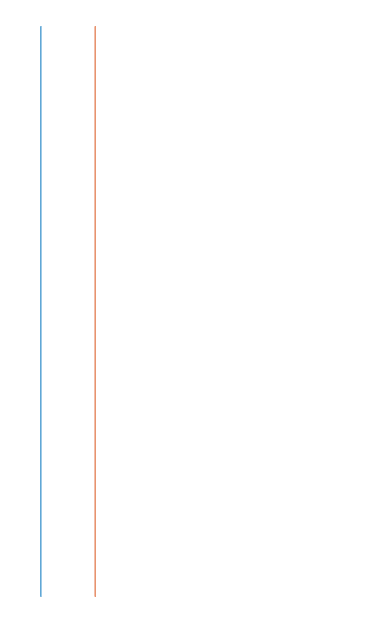
\includegraphics[width=0.15\linewidth]{pose180.png}}
\fbox{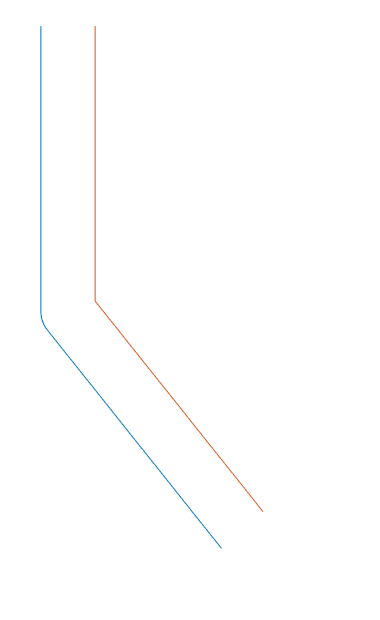
\includegraphics[width=0.15\linewidth]{pose140.png}}
\fbox{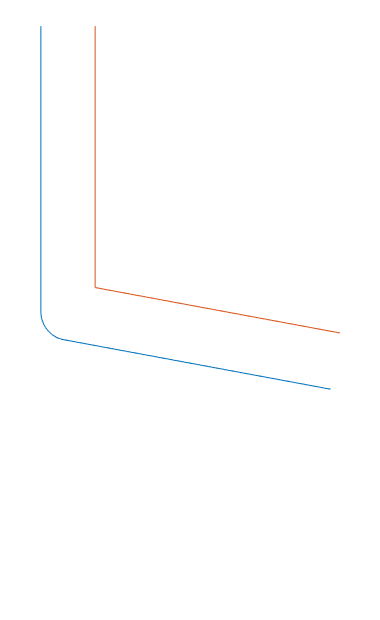
\includegraphics[width=0.15\linewidth]{pose100.png}}
\fbox{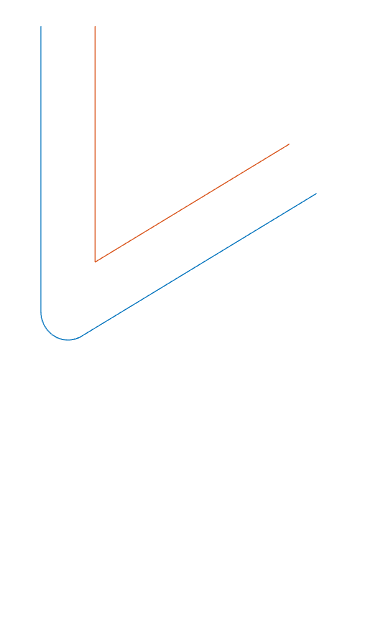
\includegraphics[width=0.15\linewidth]{pose60.png}}
\fbox{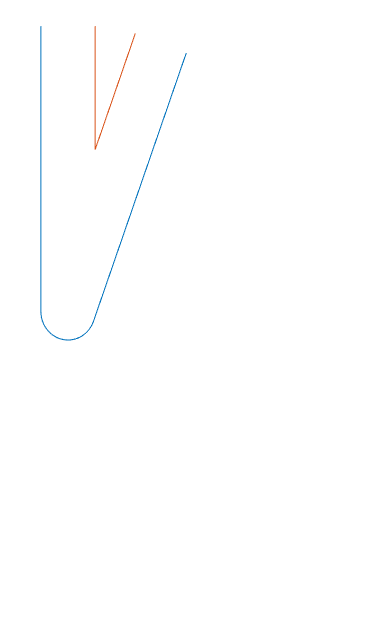
\includegraphics[width=0.15\linewidth]{pose20.png}}
\end{center}
   \caption{The five example poses defined at $\theta = 180^{\circ}, 140^{\circ}, 100^{\circ}, 60^{\circ}, 20^{\circ}$.}
\label{fig:short}
\label{poses}
\end{figure*}

%------------------------------------------------------------------------
\section{Related Work}

Weighted pose space deformation (WPSD) is an even more advanced example-based skinning method, which were derived from a hand model using medical images \cite{kurihara2004modeling}. WPSD is able to generate realistic skinning even with a limited number of poses. Lewis \cite{rhee2006real} expands on this method by implementing parallel WPSD using fragment processors. This approach only works for poses with more than one degree of freedom, so we were not able to implement WPSD with the examples used for this paper.

%------------------------------------------------------------------------
\section{Methodology}

We used MATLAB implement in code and generate images.

For the implementations of SSD and PSD in this paper, we created a simple bone structure consisting of two bones and one degree of freedom. The resulting bind pose is shown in Figure \ref{bind}. Let $\theta$ be the angle between the two bones, so that $\theta = 180^{\circ}$ in the bind pose. To test the implementations of SSD and PSD, we varied the value of $\theta$. We kept the upper bone (the blue line in Figure \ref{bind}) fixed, while moving the lower bone (the red line Figure \ref{bind}).

Joint weights needed to be defined for both SSD and PSD. Let $w(v) = (w_u, w_l)$ be defined as the weight distribution for a vertex $v$ on the skin, where $w_u$ is the weight corresponding to the upper bone and $w_l$ is the weight corresponding to the lower bone. We defined the weights to be as follows: $w(v) = (1,0)$ if $v$ is on the upper half of the upper bone, $w(v) = (0,1)$ if $v$ is on the lower half of the lower bone, $w(v)$ is a linear distribution from $(1,0)$ to $(0.5,0.5)$ for the vertices on the lower half of the upper bone, and $w(v)$ is a linear distribution from $(0.5,0.5)$ to $(0,1)$ for the vertices on the upper half of the lower bone, so that the vertex connecting the two bones has weight $(0.5,0.5)$. This setup also ensures that $w_u + w_l = 1$ for every vertex on the skin.

%------------------------------------------------------------------------
\section{Skeletal Subspace Deformation (SSD)}

The general equation for SSD is
\begin{align} v(p_a) = S(v_0) \end{align}
where $p_a$ is an arbitrary pose, $v(p_a)$ is a vertex of a deformed target of $p_a$, $v_0$ is the corresponding vertex in the bind pose, and $S$ is the SSD function.

Using the bind pose and joint weights as defined in the methodology, SSD computes the position of each skin vertex by using the weighted blending of an affine transformation of each joint from the bind pose. Then we can define $S$ to be
\begin{align} S(v_0) = (\sum_{j=1}^{n_{joint}} w_j T_j) v_0 
\label{ssd_eq}
\end{align}
where $n_{joint}$ is the number of joints, $w_j$ is the predefined joint weight, and $T_j$ is joint $j$'s transformation to the current vertex.

\begin{figure*}
\begin{center}
\fbox{
\includegraphics[width=0.15\linewidth]{ssd180.png}}
\fbox{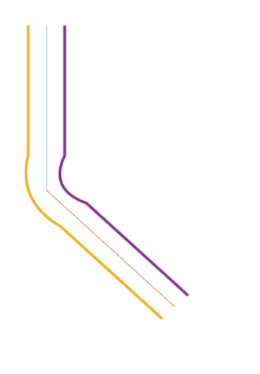
\includegraphics[width=0.15\linewidth]{ssd135.png}}
\fbox{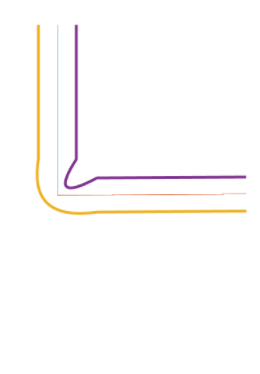
\includegraphics[width=0.15\linewidth]{ssd90.png}}
\fbox{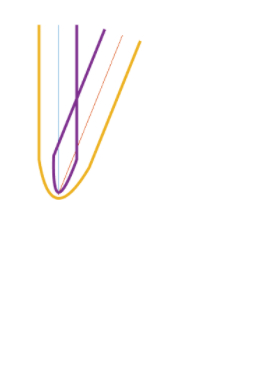
\includegraphics[width=0.15\linewidth]{ssd20.png}}
\end{center}
   \caption{The results for SSD at $\theta = 180^{\circ}, 135^{\circ}, 90^{\circ}, 20^{\circ}$.}
\label{fig:short}
\label{ssd_r}
\end{figure*}

\begin{figure*}
\begin{center}
\fbox{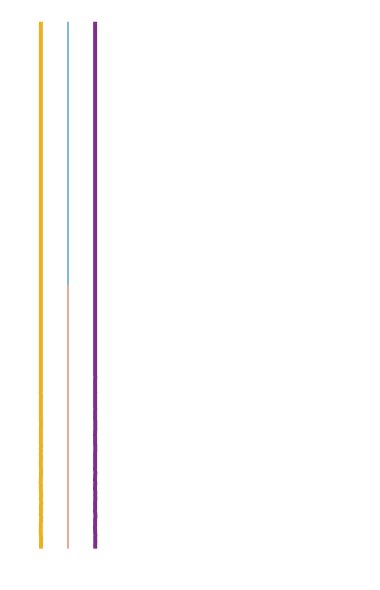
\includegraphics[width=0.15\linewidth]{psd180.png}}
\fbox{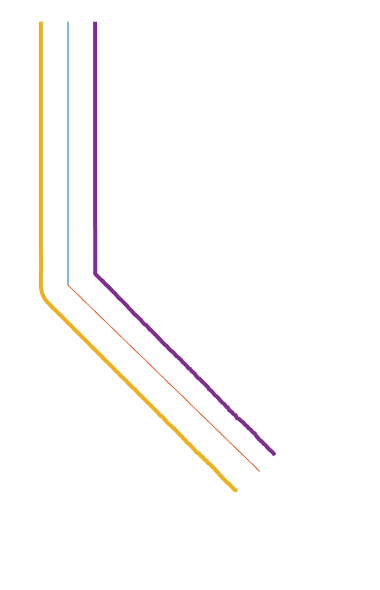
\includegraphics[width=0.15\linewidth]{psd135.png}}
\fbox{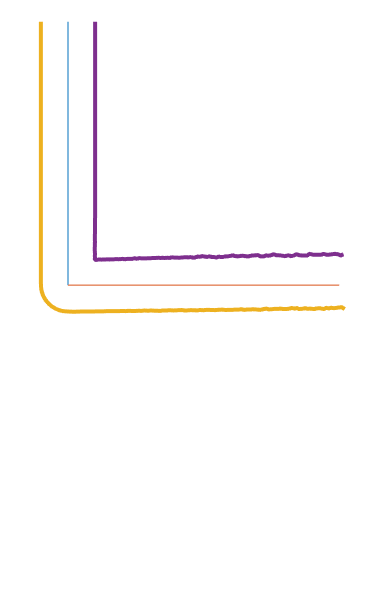
\includegraphics[width=0.15\linewidth]{psd90.png}}
\fbox{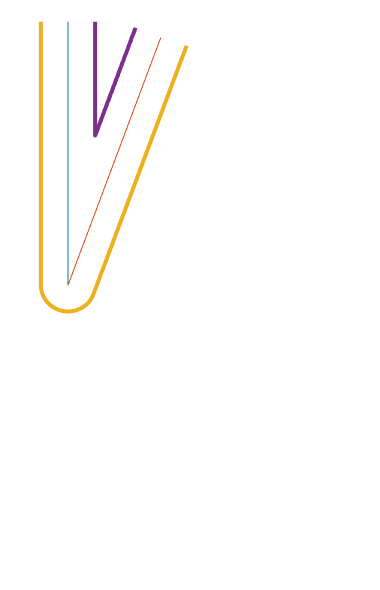
\includegraphics[width=0.15\linewidth]{psd20.png}}
\end{center}
   \caption{The results for PSD at $\theta = 180^{\circ}, 135^{\circ}, 90^{\circ}, 20^{\circ}$.}
\label{fig:short}
\label{psd_r}
\end{figure*}

%------------------------------------------------------------------------
\section{Pose Space Deformation (PSD)}

The general equation for PSD is
\begin{align} v(p_a) = S(v_0 + D(p_a)) \end{align}
where $D(p_a)$ is the displacement as a function of the arbitrary pose.

PSD requires a set of arbitrary poses to first be defined where the strange deformations happen. We defined four example poses at $\theta = 140^{\circ}, 100^{\circ}, 60^{\circ}, 20^{\circ}$. These predefined poses along with the bind pose are shown in Figure \ref{poses}. Given this set of example poses, we can interpolate to calculate $D(p_a)$ in the ``pose space'' \cite{lewis2000pose}. 

We first need to compute the displacements of the example poses in the rest coordinates to be able to interpolate on them. We can do this by using inverse SSD on each example pose $k$:
\begin{align} d_k = (\sum_{j=1}^{n_{joint}} w_j T_j)^{-1} v_k - v_0 \end{align}

We used the radial basis function \cite{lewis2000pose} to interpolate the displacement for the arbitrary pose:
\begin{align} D(p_a) = \sum_{k=1}^{n_{pose}} \lambda_k \phi(\| \mathbf{x} - \mathbf{x_k} \| ) 
\label{rbf}
\end{align}
We use Gaussian radial basis function as following
\begin{align} \phi(x) = e^{-(\epsilon x)^2} \end{align}
where $x$ is the distance. In our implementation, we use the difference in degrees.

Gaussian function converges to 0 very quickly, which ensures that displacements at an angle $\theta$ will not be affected greatly by displacements at extreme angles, e.g. at $20^{\circ}$. At the same time, we set $\epsilon$ to be fairly small so that it would not converge to 0 too quickly. By doing so, we were able to interpolate displacements for any arbitrary angle smoothly.

In our implementation, we calculated $\lambda_k$ on the fly. This is done by solving a linear system 
\begin{equation}
	D=\boldsymbol{\phi}\cdot\lambda
\end{equation} 
where displacements vector for each predefined pose $D$ is pre-computed and $\boldsymbol{\phi}$ depends on those poses. Then displacements for any arbitrary pose can be interpolated using equation \ref{rbf}.

%------------------------------------------------------------------------
\section{Computing joint weights from samples}
The joint weights of each vertex are important to generate accurate skinning in SSD (equation \ref{ssd_eq}). The joint weights of each vertex can be automatically calculated from the sample poses to enhance the accuracy of the weight value. This should result in better skinning and reduces the elaborate manual work required to create weight maps.

In each sample pose $p_k$, we have following equation based on SSD:
\begin{equation}
	\tilde{v_k}-e_k=(\sum_{j=1}^{n_{joint}}w_jT_j)v_0
\end{equation}
where $\tilde{v_k}$ is a particular vertex from skin sample $k$, the right hand side is the SSD deformation of vertex $v_0$ from the rest pose, and $e_k$ is a displacement between the SSD deformation and $\tilde{v_k}$.
If we have sufficient examples involving the same set of $n_{joint}$ joints, we have $n_{pose}$ equations of the form:
\begin{equation}
	\tilde{v_k}-e_k=\sum_{j=1}^{n_{joint}}v_jw_j
\end{equation}
where $v_j$is $v_0$ transformed by $T_j$. We can minimize the error $e_k$ using least square method
\begin{equation}
	\Arrowvert\boldsymbol{v}-\boldsymbol{Aw}\Arrowvert^2
\end{equation}
where $\boldsymbol{w}$ is a weight vector, $\boldsymbol{v}$ is the predefined pose vertex vector, and $\boldsymbol{A}$ is a transformed vertex matrix. Finally, weights are scaled to ensure that they sum up to 1.

%------------------------------------------------------------------------
\section{Results}

The results of SSD are shown in Figure \ref{ssd_r}. As expected, the result at $\theta = 180^{\circ}$ is perfect since that is the bind pose. However, for the other angles, it is very apparently that the skin collapses where the bones meet. At extreme angles like $\theta = 20^{\circ}$, the inner skin even collapses past the bone and folds into itself.

The results of PSD are shown in Figure \ref{psd_r}. (A YouTube video showing the results of PSD for $15^{\circ} \leq \theta \leq 190^{\circ}$ is also available \href{https://youtu.be/v3lwH1p3HBU}{here}). Even though some results are computed at angles that were not defined in the example poses (besides at $\theta = 180^{\circ}$), the skin does not collapse, has very smooth transitions, and stays close along the bones. This shows that PSD can deal with extreme angles and our interpolation is smooth.

The results of the computed joint weights are shown in Figure \ref{com_w}. The results do not look good because the least squares by subspace projection can produce weights that are less than 0 or greater than 1, in which case the outcome will not converge.

Another disadvantage of SSD is it cannot handle rotation in 3D. The skin collapses while rotating. However, by defining poses for different rotation angles, PSD can solve this problem easily.

PSD also is not computationally expensive. In our system, coefficients for the radial basis function are computed on the fly while it only takes $20\%$ more time than SSD. Lewis \cite{rhee2006real} tried to do real-time PSD for large meshed on GPU, which makes it even faster. 

\begin{figure}[t]
\begin{center}
\fbox{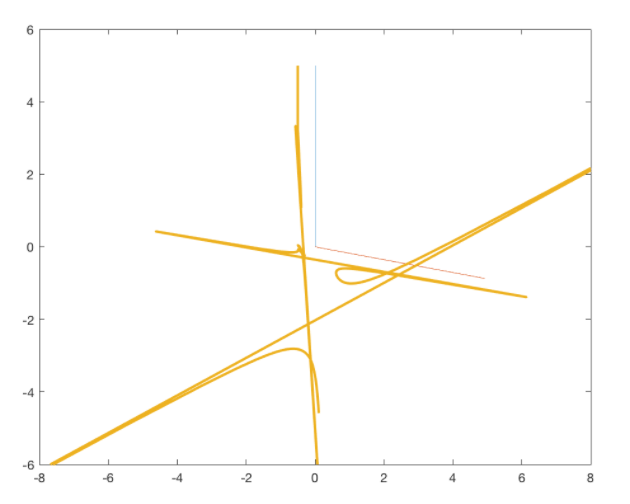
\includegraphics[width=0.8\linewidth]{computed_weights.png}}
\end{center}
   \caption{The results with computed joint weights using least squares estimation.}
\label{fig:long}
\label{fig:onecol}
\label{com_w}
\end{figure}

%------------------------------------------------------------------------
\section{Conclusion}

We were able to show the shortcomings of SSD at sharp angles and also demonstrate that, with appropriately defined example poses and appropriately chosen parameters for the radial basis function, PSD can fix those issues and produce smooth skinning.

In our simple two-bone system there was only one degree of freedom (DOF) so we could not implement WPSD \cite{kurihara2004modeling}. We can expand our system to 3D and add more DOFs. Then we can try to interpolate facial expression or to skin more arbitrary poses for characters. 

We could also try to implement the non-negative least square (NNLS) method instead of subspace projection, which may produce converged SSD and WPSD outcome.

PSD unifies two techniques that have been common in computer graphics. It uses a relatively simple algorithm and can handle a wide variety of deformations from a simple elbow in our example to secondary animation. The setup cost of the algorithm is insignificant, and the synthesis cost is only slightly more than that of shape interpolation.

%------------------------------------------------------------------------
\section*{Acknowledgements}

We would like to thank Professors Wojciech Matusik and Justin Solomon for their guidance throughout this project.

%------------------------------------------------------------------------
\bibliographystyle{unsrt}
\bibliography{reference}

\end{document}
